
%(BEGIN_QUESTION)
% Copyright 2007, Tony R. Kuphaldt, released under the Creative Commons Attribution License (v 1.0)
% This means you may do almost anything with this work of mine, so long as you give me proper credit

Suppose we ``drive'' one twisted pair of a Category-5 (``Cat-5'') communications cable with a signal generator having the same Th\'evenin equivalent impedance as the cable (100 $\Omega$, which is standard for the unshielded, twisted wire pairs Cat-5 cable).  Actually, the cable consists of two coiled sections joined together in the middle so that we may monitor voltage mid-way as well as at the front end where the signal generator connects, with a dual-trace oscilloscope:

$$\includegraphics[width=15.5cm]{i02182x01.eps}$$

Given a typical velocity factor of 0.7, meaning that electrical signals will travel down the cable at 70\% the speed of light, it should take 10 microseconds for the signal to travel from the signal generator to the far end of the cable.  Given these conditions, we input a square-wave voltage signal at a frequency of 250 Hz and record the results:

$$\includegraphics[width=15.5cm]{i02182x02.eps}$$

So far, things look just fine.  We are seeing the same voltage signal at the mid-point of the cable that we're injecting at the left-hand end.  There is no noticeable distortion, and the time delay due to propagation time along the cable length is too short to be significant at this scale.

\vskip 10pt

\filbreak

Now, we increase the signal generator frequency to 5 kHz and correspondingly increase the sweep speed of the oscilloscope.  The waveforms we see are not so clean anymore!

$$\includegraphics[width=15.5cm]{i02182x03.eps}$$

Explain what accounts for the ``stepped'' shape of the square wave on its leading and trailing edges.

\underbar{file i02182}
%(END_QUESTION)





%(BEGIN_ANSWER)

During the time period where the wave front has yet to reach the cable end and ``reflect'' back, the signal will be mid-way between the source's old voltage and the source's new voltage because the characteristic impedance of the cable manifests itself as a 100 $\Omega$ resistance between the cable's source voltage and end voltage.

\vskip 10pt

Challenge question: what do you think the signal will look like at the far-right end of the cable?

%(END_ANSWER)





%(BEGIN_NOTES)

Answer to challenge question:

$$\includegraphics[width=15.5cm]{i02182x04.eps}$$

\vskip 10pt

One detail that might be worth mentioning is that the oscilloscope would have to have isolated inputs in order for this test to work.  Otherwise, the common ground connection through both inputs (A and B) would mess things up by bypassing one wire in the twisted pair with the first 1050 meter section!

%INDEX% Electronics review: characteristic impedance of transmission line
%INDEX% Electronics review: surge impedance of transmission line

%(END_NOTES)


